\documentclass{article}[18pt]
\ProvidesPackage{format}
%Page setup
\usepackage[utf8]{inputenc}
\usepackage[margin=0.7in]{geometry}
\usepackage{parselines} 
\usepackage[english]{babel}
\usepackage{fancyhdr}
\usepackage{titlesec}
\hyphenpenalty=10000

\pagestyle{fancy}
\fancyhf{}
\rhead{Sam Robbins}
\rfoot{Page \thepage}

%Characters
\usepackage{amsmath}
\usepackage{amssymb}
\usepackage{gensymb}
\newcommand{\R}{\mathbb{R}}

%Diagrams
\usepackage{pgfplots}
\usepackage{graphicx}
\usepackage{tabularx}
\usepackage{relsize}
\pgfplotsset{width=10cm,compat=1.9}
\usepackage{float}

%Length Setting
\titlespacing\section{0pt}{14pt plus 4pt minus 2pt}{0pt plus 2pt minus 2pt}
\newlength\tindent
\setlength{\tindent}{\parindent}
\setlength{\parindent}{0pt}
\renewcommand{\indent}{\hspace*{\tindent}}

%Programming Font
\usepackage{courier}
\usepackage{listings}
\usepackage{pxfonts}

%Lists
\usepackage{enumerate}
\usepackage{enumitem}

% Networks Macro
\usepackage{tikz}


% Commands for files converted using pandoc
\providecommand{\tightlist}{%
	\setlength{\itemsep}{0pt}\setlength{\parskip}{0pt}}
\usepackage{hyperref}

% Get nice commands for floor and ceil
\usepackage{mathtools}
\DeclarePairedDelimiter{\ceil}{\lceil}{\rceil}
\DeclarePairedDelimiter{\floor}{\lfloor}{\rfloor}

% Allow itemize to go up to 20 levels deep (just change the number if you need more you madman)
\usepackage{enumitem}
\setlistdepth{20}
\renewlist{itemize}{itemize}{20}

% initially, use dots for all levels
\setlist[itemize]{label=$\cdot$}

% customize the first 3 levels
\setlist[itemize,1]{label=\textbullet}
\setlist[itemize,2]{label=--}
\setlist[itemize,3]{label=*}

% Definition and Important Stuff
% Important stuff
\usepackage[framemethod=TikZ]{mdframed}

\newcounter{theo}[section]\setcounter{theo}{0}
\renewcommand{\thetheo}{\arabic{section}.\arabic{theo}}
\newenvironment{important}[1][]{%
	\refstepcounter{theo}%
	\ifstrempty{#1}%
	{\mdfsetup{%
			frametitle={%
				\tikz[baseline=(current bounding box.east),outer sep=0pt]
				\node[anchor=east,rectangle,fill=red!50]
				{\strut Important};}}
	}%
	{\mdfsetup{%
			frametitle={%
				\tikz[baseline=(current bounding box.east),outer sep=0pt]
				\node[anchor=east,rectangle,fill=red!50]
				{\strut Important:~#1};}}%
	}%
	\mdfsetup{innertopmargin=10pt,linecolor=red!50,%
		linewidth=2pt,topline=true,%
		frametitleaboveskip=\dimexpr-\ht\strutbox\relax
	}
	\begin{mdframed}[]\relax%
		\centering
		}{\end{mdframed}}



\newcounter{lem}[section]\setcounter{lem}{0}
\renewcommand{\thelem}{\arabic{section}.\arabic{lem}}
\newenvironment{defin}[1][]{%
	\refstepcounter{lem}%
	\ifstrempty{#1}%
	{\mdfsetup{%
			frametitle={%
				\tikz[baseline=(current bounding box.east),outer sep=0pt]
				\node[anchor=east,rectangle,fill=blue!20]
				{\strut Definition};}}
	}%
	{\mdfsetup{%
			frametitle={%
				\tikz[baseline=(current bounding box.east),outer sep=0pt]
				\node[anchor=east,rectangle,fill=blue!20]
				{\strut Definition:~#1};}}%
	}%
	\mdfsetup{innertopmargin=10pt,linecolor=blue!20,%
		linewidth=2pt,topline=true,%
		frametitleaboveskip=\dimexpr-\ht\strutbox\relax
	}
	\begin{mdframed}[]\relax%
		\centering
		}{\end{mdframed}}
\lhead{Computational Thinking}


\begin{document}
\begin{center}
\underline{\Large How do we know that an algorithm solves a particular problem?}
\end{center}
\section{Software Bugs}
\begin{itemize}
	\item \textbf{Software Bug} - An error in the program that causes the program to behave in an unintended or an unexpected way
	\item This usually arises from the programmer's error, but can arise because of a "secondary error" - such as a poorly written complier
\end{itemize}
Bugs can affect programs in various ways
\begin{itemize}
	\item Produce incorrect results
	\item Program crashes
	\item Susceptible to malicious attack
	\item Runs slowly or gobbles up memory
\end{itemize}
\section{How do we get bug free software?}
\begin{itemize}
	\item \textbf{Software Engineering} - The application of a systematic, disciplined and quantifiable approach to the development, operation and maintenance of the software
\end{itemize}
The 5 phases of the waterfall model:
\begin{itemize}
	\item \textbf{requirements phase} - where the specification of what the program is intended to do is produced
	\item \textbf{design phase} - where a plan is composed for the intended solution and where this plan involves algorithms and their implementations, architectural aspects, data structures and so on
	\item \textbf{implementation phase} - where the design is implemented as code
	\item \textbf{verification phase} - where the code is tested and debugged
	\item \textbf{maintenance phase} - the continual updating and modifying of the code
\end{itemize}
\section{Establishing correctness: software testing vs formal methods}
\textbf{Software testing} - The process of evaluating an attribute or capability of a program or system\\
The phases of the process of software testing:
\begin{itemize}
	\item Modelling the program's environment so that the program will be tested under conditions as near as possible to those for which the program has been designed
	\item Selecting test scenarios so as to try and achieve as good a coverage as possible 
	\item Running and evaluating test scenarios, preferably in an automated fashion
	\item Measuring test progress
\end{itemize}
The problem with this method is that it depends on the tests you pick, there may be a set of inputs that you haven't used that would cause an error.\\
\\
One way to test this is through an alpha or beta test, this will mean that users will do huge sets of inputs, and will likely find any bugs that exist\\
\\
\textbf{Formal Methods:} Use mathematically based techniques to formally specify and formally verify software and hardware systems
\begin{itemize}
	\item More concerned with correctness than implementation
	\item Two fundamental activities - specification and verification
	\item The specification is derived as a collection of logical formulae
	\item Mathematical techniques are sometimes used to convert the specification into a program so that it can be verified mathematically
	\item Formal methods are closely linked with automated theorem proving, where programs are developed to automatically prove mathematical theorems
	\item They are also linked to model checking, where properties of specifications are automatically evaluated using model checking software
\end{itemize}
Some argue that the expense, time and skills required for formal techniques are not merited. However if safety critical operations, formal methods will give the more accurate result, so is the better option. \\
\\
\textbf{Software metric} - A measure if testing hardness
\begin{itemize}
	\item How sensible/efficient do you want code?
	\item How much time and money to spend before giving up?
	\item Two main metrics
	\begin{itemize}
		\item Lines of code - only eliminate a certain number of bugs per certain lines of code
		\item Cyclotomic complexity - How many paths through the code are there? Find core paths and get them bug free, more unused paths may have some bugs left in
	\end{itemize}
\end{itemize}
\section{What do we mean by correct?}
\textbf{Totally Correct} - Correct with respect to some specification and terminates on every input\\
\textbf{Partially Correct} - Only correct with respect to the specification, no guarantee of termination\\
\\
\textbf{Assertions} are used to check if conditions hold of variables etc, for example if a variable 0 when it should be etc.
\section{Factorial Induction}
\subsection{Recursion}
\begin{itemize}
	\item \textbf{Base case} - When the value of y is 0 - terminates and is correct
	\item \textbf{Inductive step}
	\begin{itemize}
		\item Assume P(n) for some $n\geqslant 0$, that is, factorial(y) terminates and is correct whenever we have the input value os y is $\geqslant 0$ and $\leqslant$ n
		\item Factorial(y) with the input value of y given as $(n+1)>0$
		\begin{itemize}
			\item Induction Holds yeilds termination and that it computes $(n+1)!$
		\end{itemize}
	\end{itemize}
\end{itemize}
\subsection{Iteration}
\begin{itemize}
	\item \textbf{Termination}
	\begin{itemize}
		\item Observation: y decreases by 1 at the end of every iteration of the while loop
		\item So there are n iterations of the while loop and we have termination
	\end{itemize}
	\item \textbf{Correctness}
	\begin{itemize}
		\item n-y+1 increases by 1 at the end of each iteration of the while loop
		\item Prior to the first execution of the while loop n-y+1 has value 1
		\item observation: during the ith iteration, x is multiplied by y
		\item Our algorithm outputs n! after n iterations
	\end{itemize}
\end{itemize}



\section{More complicated inductions}
Consider $\Pi =\{(a,b): a\geqslant b\geqslant 0\}$\\
Define the lexicographic ordering on this set $\Pi$
\begin{itemize}
	\item $(a,b)=(c,d)$ if, and only if, a=c and b=d
	\item $(a,b)>(c,d)$ if, and only if, either $a>c$ or $(a=c and b>d)$
\end{itemize}
So, the pairs in $\Pi$ can be ordered as
$$\begin{array} { l } { ( 0,0 ) < ( 1,0 ) < ( 1,1 ) < ( 2,0 ) < ( 2,1 ) < ( 2,2 ) < ( 3,0 ) } \\ { \quad < ( 3,1 ) < ( 3,2 ) < ( 3,3 ) < ( 4,0 ) < \ldots } \end{array}$$
Suppose that some property P is indexed by pairs $(a,b)\in \Pi$. We can undertake induction as follows
\begin{itemize}
	\item \textbf{Base Case}: Show that $P(0,0)$ holds (or in general, $P(a_0,b_0)$, for some $a_0\geqslant b_0\geqslant 0)$
	\item \textbf{Inductive step:} Assume that $P(a,b)$ is true for some $(a,b)$ where $a\geqslant b\geqslant 0$ ( in general, where $(a,b)\geqslant (a_0,b_0)$ in the lexiographic ordering). We then prove that if this is the case then $P(a_+,b_+)$ is the next pair in the lexiographic ordering after $(a,b)$
	\item \textbf{Principle of induction:} allows us to state that $P(a,b)$ holds for all $a\geqslant b\geqslant 0$ (in general, when $(a,b)\geqslant (a_0,b_0)$) 
\end{itemize}
There is nothing clever going on here. What we are really doing is working with the property $Q(n)$ which is the property '$P(a,b)$ where $(a,b)$ is the nth pair in the lexiographic ordering of $\Pi$'
\subsection{In lecture}
\begin{itemize}
	\item 
\end{itemize}




\section{Euclid's algorithm}
\subsection{Recursively}
Recall the recursive version of Euclid's algorithm, namely Euclid(x,y), where we assume that initially x=m and y=n with $(m,n)\in \Pi \backslash \{(0,0)\}$
\begin{center}
	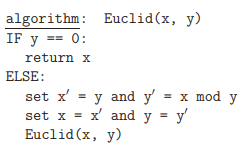
\includegraphics[scale=0.7]{euclid}
\end{center}
We can use our extended principle of induction to prove total correctness. We would also like to use induction as follows: 'our induction hypothesis tells us that any recursive call to Euclid is totally correct; so, our main call to euclid must be totally correct'\\
We begin with an observation: if Euclid(x,y) is called with the value of (x,y) being $(a,b)\in \Pi \backslash \{(0,0)\}$ and if Euclid(x,y) is then called recursively with the value of (x,y) being $(a',b')$ (so, necessarily $b>0$ in order for this recursive call to occur) then we must have that:
\subsection{In lecture}
\begin{itemize}
	\item Call euclid with 2 inputs m and n greater than 0 where $a\geqslant b$ and if euclid(m,n) is subsequently called recursively with the value of (m,n) being $(a',b')$
	\item $(a',b')>(0,0)$ and $a'\geqslant b'$
	\item $(a,b)>(a',b')$
	\item So, the values obtained tracking consecutive values of (m,n) are decreasing and so will eventually reach 0, after which the algorithm will terminate
\end{itemize}
Induction
\begin{itemize}
	\item \textbf{Base case} - m=1 and n=0 - algorithm terminates and is correct
	\item \textbf{Inductive step: assume P(m,n)}
	\begin{itemize}
		\item Let $(m_+,n_+)$ be the successor of (m,n) in the lexiographic order
		\item If $n_+=0$ then we are done
		\item If $n_=>0$ then we make the recursive call of euclid$(n_+,m_+ mod n_+)$ and as these values are no bigger than before, moving towards the base case, and so will terminate correctly
	\end{itemize}
\end{itemize}
\subsection{Iteratively}
\begin{itemize}
	\item \textbf{Termination}: Set a check point immediately prior to the execution of the while test
	\begin{itemize}
		\item At consecutive check points
		\begin{itemize}
			\item Find the pattern in what happens $(m,n)>(0,0)$ and $m>n$
			\item The value is strictly decreasing
		\end{itemize}
	\end{itemize}
	\item \textbf{Correctness}
	\begin{itemize}
		\item Suppose that initially m and n are u and v respectively, and m has value w on termination
		\item Two possibilities, swap or not, one value reduces and one swaps
		\item So an integer x divides both $u_1$ and $v_1$ iff x divides both $u_2$ and $v_2$
		\item Eventually x will divide w and 0, and so the answer will be correct
	\end{itemize}
\end{itemize}
\section{Invariants}
\begin{itemize}
	\item A property that is always true at some given check point in an algorithms execution (usually prior to a loop test)
\end{itemize}
Easiest to see in rewriting of iterative algorithms\\
Copy algorithms in
\end{document}